\documentclass[a4paper,10pt]{article}

\usepackage[margin=1in]{geometry}
\usepackage{amsmath,amsthm,amssymb,hyperref}
%% For subfigure
\usepackage{caption,subcaption,graphicx}

\hypersetup{colorlinks=true,urlcolor=blue}

\usepackage{embedfile,fancyvrb}
\embedfile{\jobname.tex}

\usepackage{fancyhdr}
\pagestyle{fancy}
\lhead{Danny Hermes}
\rhead{Brad Poopy Head}

\renewcommand{\headrulewidth}{0pt}

\begin{document}

\textbf{NOTE:} To extract the \LaTeX\ source of this PDF and the supporting
files, execute:
\begin{Verbatim}[commandchars=\\\{\}]
pdftk \jobname.pdf unpack_files output .
\end{Verbatim}

We want to parameterize the three shapes so we can easily understand
what is happening. We assume the top of the sphere is \(0.3 \mu m\) away
from the horizontal cylinder, the sphere has a radius of \(0.1 \mu m\), the
vertical cylinder (dendrite) has diameter \(0.1 \mu m\) and the ``main line''
horizontal cylinder (that all the dendrites come out of has a diameter) of
\(1.0 \mu m\). We can visualize a cross-section of the top part via
\begin{verbatim}
H = 0.5;
theta = 0:0.01:(2*pi);
sphereIn2D = [0.1*cos(theta); 0.1*sin(theta) + 0.2 + H];

vertY = H:0.001:(H + 0.15);
leftPoints = [-0.05 * ones(size(vertY)); vertY];
rightPoints = [0.05 * ones(size(vertY)); vertY];
verticalCylinder = [leftPoints, rightPoints];

horizontalX = -0.3:0.001:0.3;
horizontalCylinder = [horizontalX; H * ones(size(horizontalX))];

allPoints = [sphereIn2D, verticalCylinder, horizontalCylinder];
scatter(allPoints(1, :), allPoints(2, :));
axis equal;

axis([-0.5, 0.5, 0.3, 1])
\end{verbatim}

\begin{figure}
  \centering
    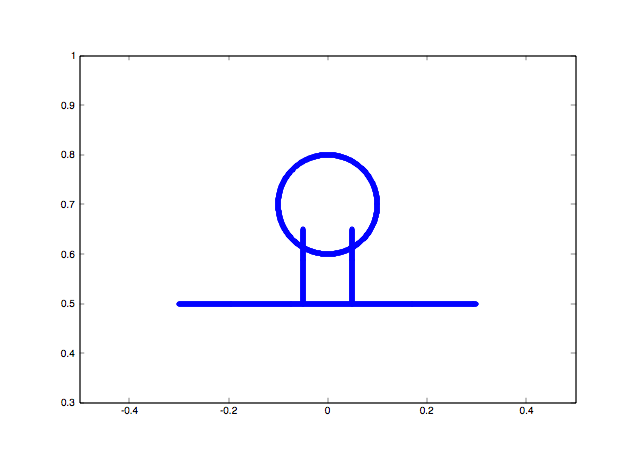
\includegraphics[scale=0.3]{cross_section.png}
  \caption{Cross-Section of Dendrite}
  \label{fig:1a}
\end{figure}

and see in Figure~\ref{fig:1a} the general cross-sectional geometry.

We need to find intersection points, but first get a basic idea of
the equations describing them:
\begin{itemize}
\item Top-Sphere: \(x^2 + y^2 + \left(z - 0.7\right)^2 = 0.1^2\). This has
a diameter of \(0.2 \mu m\) and has to be \(0.3 \mu m\) above the main
(horizontal) cylinder which is already \(0.5 \mu m\) above \(z = 0\), hence
we assume the center lies at \((0, 0, 0.5 + 0.3 - 0.1)
= (0, 0, 0.7)\) (since the radius is \(0.1\)).
\item Vertical Cylinder: \(x^2 + y^2 = \left(\frac{0.1}{2}\right)^2 =
0.05^2\). This is simply a circle of diameter \(0.1\) that extends infinitely
in the \(z\)-direction. This is assumed to be centered around \((x, y)
= (0, 0)\) but may change the \(x\) position of the center as we consider
dendrites on the left and/or right.
\item Horizontal Cylinder: \(y^2 + z^2 = \left(\frac{1.0}{2}\right)^2 =
0.5^2\). This is simply a circle of diameter \(0.1\) that extends infinitely
in the \(x\)-direction. This is the ``main line'' that all dendrites
sprout out of.
\end{itemize}

\textbf{Intersection points}: To find places where our geometries intersect
we need to find simultaneous solutions to the equations defining the
surfaces. For the intersection of the sphere and the dendrite cylinder,
we have
\[0.1^2 = x^2 + y^2 + \left(z - 0.7\right)^2 = 0.05^2 + \left(z -
0.7\right)^2.\]
This gives us
\[\left(z - 0.7\right)^2 = 0.0075 \Rightarrow z = 0.7 \pm \sqrt{0.0075}.\]
However, the top one of these points corresponds to an intersection of our
cylinder that is irrelevant to our geometry hence we can say that \(z =
0.7 - \sqrt{0.0075}\) uniquely. This gives us the first rule for determining
if a point changes geometries:
\[\boxed{\text{if } z \geq 0.7 - \sqrt{0.0075} \text{ the point is on the
sphere, else it below}}\]

To determine the other intersection, we want to find the curve that is
the intersection of the surfaces given by
\[x^2 + y^2 = 0.05^2 \quad \text{ and } \quad y^2 + z^2 = 0.5^2\]
We can think of this as a parametric curve where \(z\) is the parameter.
On the first surface we must have \(0 \leq x, y \leq 0.05\) hence in the
second we see that
\[0.2475 = 0.5^2 - 0.05^2 \leq z^2 = 0.5^2 - y^2 \leq 0.5^2 - 0^2 = 0.25.\]
Since our cylinders only intersect in the top half of the plane (i.e. the
dendrites don't sprout on both sides) we only consider the positive
\(z\)-values:
\[\sqrt{0.2475} \leq z \leq 0.5.\]
Given such a \(z\)-value we have \(y^2 = 0.25 - z^2\) and \(x^2 = 0.0025 -
y^2 = z^2 - 0.2475\). Hence our parameterization results in four curves:
\[\left(\pm \sqrt{z^2 - 0.2475}, \pm \sqrt{0.25 - z^2}, z\right).\]

\begin{figure}
  \centering
  %%
  \begin{subfigure}{.45\textwidth}
    \centering
      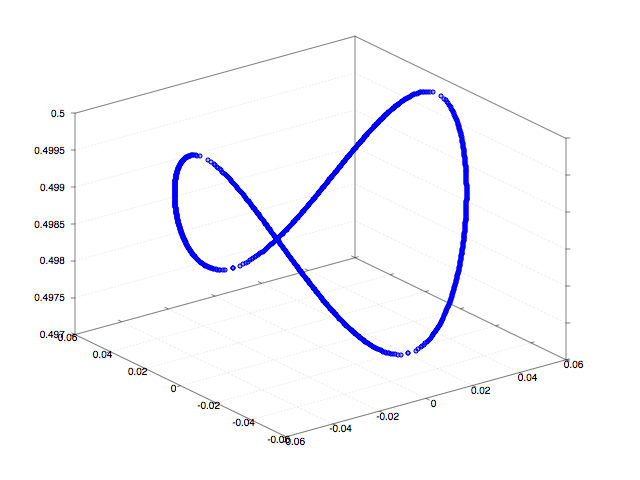
\includegraphics[width=\linewidth]{cylinder_intersection_pringle.png}
    \caption{Pringle}
    \label{fig:1b-a}
  \end{subfigure}
  %%
  \begin{subfigure}{.45\textwidth}
    \centering
      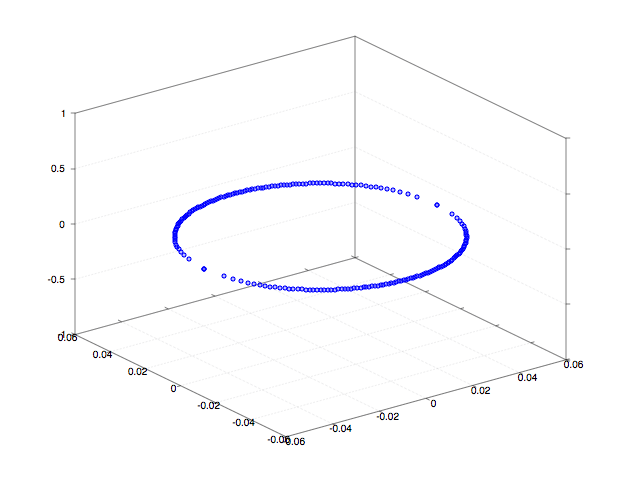
\includegraphics[width=\linewidth]{cylinder_intersection_domain.png}
    \caption{\(z\)-agnostic domain}
    \label{fig:1b-b}
  \end{subfigure}
  %%
  \caption{Intersection of Cylinders}
  \label{fig:1b}
\end{figure}

Plotting this via
\begin{verbatim}
z = sqrt(1/4 - 1/400):0.00001:sqrt(1/4);
x = sqrt(z.*z - 99/400);
y = sqrt(1/4 - z.*z);
pts1 = [x; y; z];
pts2 = [-x; y; z];
pts3 = [x; -y; z];
pts4 = [-x; -y; z];
pts = [pts1, pts2, pts3, pts4];

otherx = -sqrt(1/400):0.001:sqrt(1/400);
othery = sqrt(max(1/400 - otherx.*otherx, 0));
otherpts1 = [otherx; othery; zeros(size(otherx))];
otherpts2 = [otherx; -othery; zeros(size(otherx))];
otherpts = [otherpts1, otherpts2];

scatter3(pts(1, :), pts(2, :), pts(3, :));
figure;
scatter3(otherpts(1, :), otherpts(2, :), otherpts(3, :));
\end{verbatim}
we see in Figure~\ref{fig:1b} that the intersection is a ``pringle'' shape.

From this it's clear that points with \(z > 0.5\) (and also below
\(0.7 - \sqrt{0.0075}\), where the sphere ends) must be on the dendrite.
Also points with \(z < \sqrt{0.2475}\) must be on the ``main line''. However
points in between can be on either one. For such points, we must also know
the \(x, y\) values. If \(x^2 + y^2 > 0.05^2\), then the point must be on
the main line. If \(x^2 + y^2 < 0.05^2\), then it must be thrown away ---
this would be a part of the ``main line'' cylinder covered up by the interior
of the dendrite cylinder. If \(x^2 + y^2 = 0.05^2\) then it lies on the
dendrite. For points on the dendrite, if \(y^2 + z^2 < 0.5^2\), then we
discard the point.

Using
\begin{verbatim}
theta = 0:0.05:(2*pi);
r = 0.05;
xPoints = r * cos(theta);
yPoints = r * sin(theta);
zPoints = sqrt(0.2475):0.0001:0.505;
duplicateX = transpose(xPoints) * ones(size(zPoints));
duplicateY = transpose(yPoints) * ones(size(zPoints));
duplicateZ = ones(size(transpose(xPoints))) * zPoints;

duplicateX = reshape(duplicateX, 1, numel(duplicateX));
duplicateY = reshape(duplicateY, 1, numel(duplicateY));
duplicateZ = reshape(duplicateZ, 1, numel(duplicateZ));

cylinderPoints = [duplicateX; duplicateY; duplicateZ];
ysqPluszSq = (cylinderPoints.^2)(2, :) + (cylinderPoints.^2)(3, :);
goodIndices = (ysqPluszSq > 0.5^2);
cylinderPoints = cylinderPoints(:, goodIndices);

scatter3(cylinderPoints(1, :), cylinderPoints(2, :), cylinderPoints(3, :));
\end{verbatim}
we see in Figure~\ref{fig:1c} the shape of the dendrite at the boundary
using this rule.

We similarly crop the main line part using
\begin{verbatim}
theta = -pi/10:0.005:pi/10;
r = 0.5;
xPoints = -0.06:0.003:0.06;
yPoints = r * sin(theta);
zPoints = r * cos(theta);

duplicateX = ones(size(transpose(yPoints))) * xPoints;
duplicateY = transpose(yPoints) * ones(size(xPoints));
duplicateZ = transpose(zPoints) * ones(size(xPoints));

duplicateX = reshape(duplicateX, 1, numel(duplicateX));
duplicateY = reshape(duplicateY, 1, numel(duplicateY));
duplicateZ = reshape(duplicateZ, 1, numel(duplicateZ));

mainCylinderPoints = [duplicateX; duplicateY; duplicateZ];
xsqPlusySq = (mainCylinderPoints.^2)(1, :) + (mainCylinderPoints.^2)(2, :);
goodIndices = (xsqPlusySq > 0.05^2);
mainCylinderPoints = mainCylinderPoints(:, goodIndices);

scatter3(mainCylinderPoints(1, :), mainCylinderPoints(2, :), ...
         mainCylinderPoints(3, :));
\end{verbatim}
and produce Figure~\ref{fig:1d}.

\begin{figure}
  \centering
    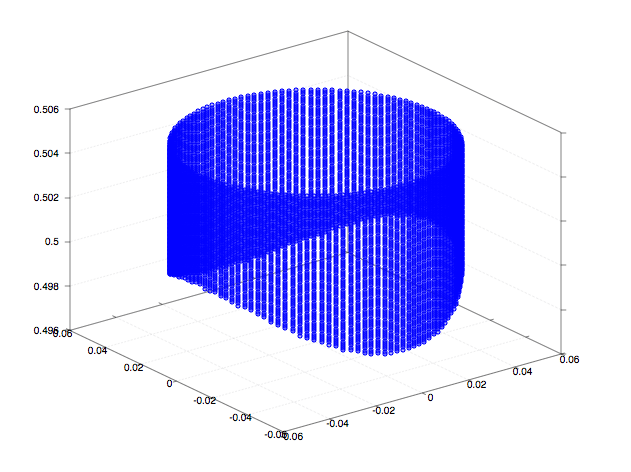
\includegraphics[scale=0.5]{top_part_dendrite.png}
  \caption{Dendrite above Main Line}
  \label{fig:1c}
\end{figure}

\begin{figure}
  \centering
    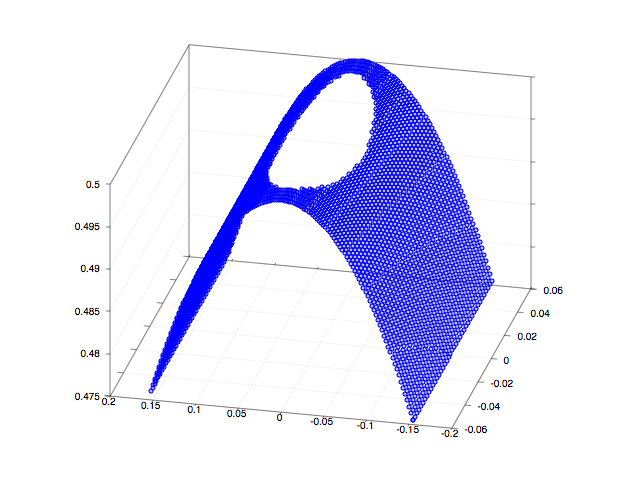
\includegraphics[scale=0.5]{cropped_main_line}
  \caption{Cropped Main Line}
  \label{fig:1d}
\end{figure}

\begin{figure}
  \centering
    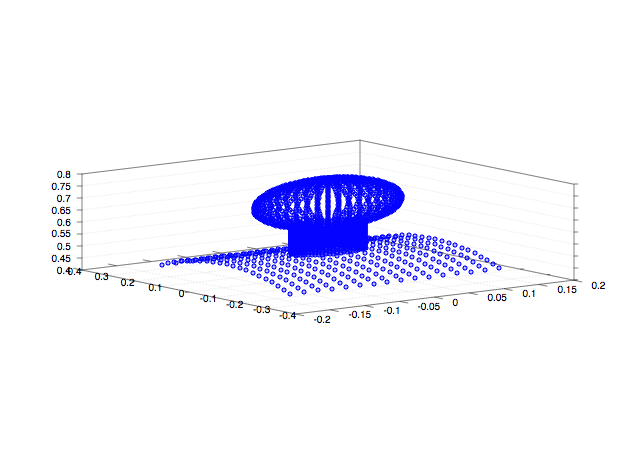
\includegraphics[scale=0.5]{whole_phenomenon.png}
  \caption{Complete Picture}
  \label{fig:1e}
\end{figure}

Using
\begin{verbatim}
theta = pi/2:0.1:pi;
phi = 0:0.15:(2*pi);
r = 0.1;

x = r * transpose(sin(theta)) * cos(phi);
x = reshape(x, 1, numel(x));

y = r * transpose(sin(theta)) * sin(phi);
y = reshape(y, 1, numel(y));

z = r * transpose(cos(theta)) * ones(size(phi));
z = 0.7 + reshape(z, 1, numel(z));

goodIndices = (z > 0.7 - sqrt(0.0075));
x = x(goodIndices);
y = y(goodIndices);
z = z(goodIndices);

spherePts = [x;y;z];

%% Do the dendrite
theta = 0:0.1:(2*pi);
r = 0.05;
xPoints = r * cos(theta);
yPoints = r * sin(theta);
zPoints = sqrt(0.2475):0.007:(0.7 - sqrt(0.0075));
duplicateX = transpose(xPoints) * ones(size(zPoints));
duplicateY = transpose(yPoints) * ones(size(zPoints));
duplicateZ = ones(size(transpose(xPoints))) * zPoints;

duplicateX = reshape(duplicateX, 1, numel(duplicateX));
duplicateY = reshape(duplicateY, 1, numel(duplicateY));
duplicateZ = reshape(duplicateZ, 1, numel(duplicateZ));

cylinderPoints = [duplicateX; duplicateY; duplicateZ];
ysqPluszSq = (cylinderPoints.^2)(2, :) + (cylinderPoints.^2)(3, :);
goodIndices = (ysqPluszSq > 0.5^2);
cylinderPoints = cylinderPoints(:, goodIndices);

%% Do the Main Line
theta = -pi/6:0.05:pi/6;
r = 0.5;
xPoints = -0.15:0.02:0.15;
yPoints = r * sin(theta);
zPoints = r * cos(theta);

duplicateX = ones(size(transpose(yPoints))) * xPoints;
duplicateY = transpose(yPoints) * ones(size(xPoints));
duplicateZ = transpose(zPoints) * ones(size(xPoints));

duplicateX = reshape(duplicateX, 1, numel(duplicateX));
duplicateY = reshape(duplicateY, 1, numel(duplicateY));
duplicateZ = reshape(duplicateZ, 1, numel(duplicateZ));

mainCylinderPoints = [duplicateX; duplicateY; duplicateZ];
xsqPlusySq = (mainCylinderPoints.^2)(1, :) + (mainCylinderPoints.^2)(2, :);
goodIndices = (xsqPlusySq > 0.05^2);
mainCylinderPoints = mainCylinderPoints(:, goodIndices);

%% Plot the whole thing
allPts = [spherePts, cylinderPoints, mainCylinderPoints];
scatter3(allPts(1, :), allPts(2, :), allPts(3, :));
axis equal;
\end{verbatim}
we are able to bring this all together as in Figure~\ref{fig:1e}.

%% http://timmurphy.org/2009/08/15/drawing-horizontal-lines-in-latex/
\begin{center}
\line(1,0){400}
\end{center}

\textbf{Moving Particles} To move on the sphere we need to flatten out the
surface \textbf{around} our current point \(p_0\).

To cover this we first consider the unit sphere centered at the origin.
We consider ourselves to be standing in front of the point \(p_0 = (x_0,
y_0, z_0)\) looking at it and have our feet on ``the ground'' so that
\(z > 0\) still corresponds to up. If \(p_0 = (0, 0, 1)\) is the north pole,
we can't stand in front and have our feet on the ground so we consider that
later as a special case. This is also true for the south pole but in our
geometry the bottom of the sphere is cut off so we ignore the south pole.

Given \(p_0\), we want to think of our scene as we would if we were
standing at \(p_0 = (0, -1, 0)\). Using
\begin{verbatim}
points = [
  0, 0, 0, 1;
  1, -1, 0, 0;
  0, 0, 1, 0
]
colors = [
   1, 0, 0;
   1, 1, 0;
   0, 1, 0;
   0, 0, 1;
]
scatter3(points(1, :), points(2, :), points(3, :), [], colors);
axis([-1, 1, -1, 1, -1, 1]);
xlabel('x'); ylabel('y'); zlabel('z');
\end{verbatim}
\begin{figure}
  \centering
    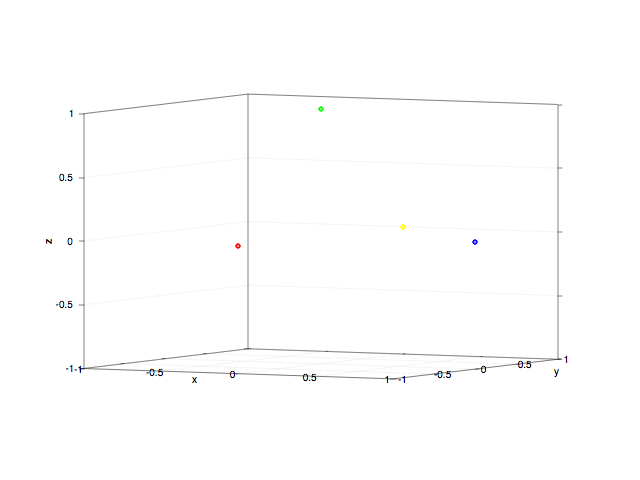
\includegraphics[scale=0.5]{standard_orientation.png}
  \caption{Standard Orientation}
  \label{fig:1f}
\end{figure}
we create Figure~\ref{fig:1f}. In it, we see \((0, -1, 0)\) as our red
viewpoint and \((0, 1, 0)\) as the yellow opposite. Given this, the green
\((0, 0, 1)\) is the ``up'' point and the blue \((1, 0, 0)\) is the right
point. We seek to find equivalent points for any given \(p_0\) (except for
the north pole).

To find the up point, we want to find a point in the same vertical plane
that \(p_0\) is in. Since a vertical plane is independent of \(z\), this
plane is simply determined by the line \(y_0 x - x_0 y = 0\) in \(3\)-space.
Given such a point \(p_1 = (a, b, c)\) we also it to be perpendicular to
\(p_0\) and of course want it to lie on the sphere. All together this
gives three conditions:
\begin{align*}
y_0 a - x_0 b &= 0 \\
a x_0 + b y_0 + c z_0 &= 0 \\
a^2 + b^2 + c^2 &= 1
\end{align*}
Solving this in Mathematica
\begin{verbatim}
soln = Simplify[Solve[a Subscript[x, 0] + b Subscript[y, 0] + c Subscript[z, 0] == 0 &&
                      a^2 + b^2 + c^2 == 1 &&
                      a Subscript[y, 0] == b Subscript[x, 0],
                      {a, b, c}],
                Subscript[x, 0]^2 + Subscript[y, 0]^2 + Subscript[z, 0]^2 == 1]
a = soln[[1, 1, 2]]
b = soln[[1, 2, 2]]
c = soln[[1, 3, 2]]
Subscript[p, 0] = {Subscript[x, 0], Subscript[y, 0], Subscript[z, 0]}
Subscript[p, 1] = {a, b, c}
\end{verbatim}
It turns out the two solutions of the system are \((a, b, c)\) and \((-a,
-b, -c)\) but since we are standing on the ground and we want the ``up''
point (the green point) we pick the solution with positive \(z\)-coordinate.
This corresponds to
\[p_1 = \left(-\frac{x_0 z_0}{\sqrt{1 - z_0^2}},
-\frac{y_0 z_0}{\sqrt{1 - z_0^2}}, \sqrt{1 - z_0^2}\right).\]
To find the ``right'' point (the blue point) we use the cross product
\(p_2 = p_1 \times p_0\) since by the
\href{http://en.wikipedia.org/wiki/Right-hand_rule}{right-hand rule} we
want the ``index finger'' to point at us, which is the direction of
\(p_0\), hence it is the second element. Actually computing this we have
\begin{verbatim}
Subscript[p, 2] = Cross[Subscript[p, 1], Subscript[p, 0]]
\end{verbatim}
which gives
\[p_2 = \left(-\frac{y_0}{\sqrt{1 - z_0^2}}, \frac{x_0}{\sqrt{1 - z_0^2}},
0\right).\]

Moving a distance \(L > 0\) at an angle of \(\theta\) from the positive
\(x\)-axis, we know we have a displacement of \((L \cos \theta, L
\sin \theta)\). This is really
\[L \cos \theta \cdot e_{\text{right}} + L \sin \theta \cdot
e_{\text{up}}.\]
where \(e_{\text{right}}, e_{\text{up}}\) are vectors in the right and up
direction. The same sort of thing happens for our points, which move in
a flattend out version of the sphere except we have
\(e_{\text{right}} = p_2\) and \(e_{\text{up}} = p_1\).

The distance along the sphere from \(p_0\) to \(p_1\) (or any other pair)
is a quarter of the circumference since \(p_1\) lies half way between
\(p_0\) and \(-p_0\) along an equator. Thus, cutting the sphere at the
equator containing \(p_1\) and \(p_2\) we get a circle with center at
\(p_0\) and a radius of \(\frac{2 \pi R}{4} = \frac{\pi}{2}\) (since we
have \(R = 1\) on the unit sphere). If we move in a direction of \(\theta\),
we could cross the point
\[p_{\theta} = \left(\cos \theta\right) p_2 + \left(\sin \theta\right) p_1\]
along the equator through \(p_1\) and \(p_2\). (This is true independent
of \(R\).) To travel a distance of
\(L\) along the equator from \(p_0\) to \(p_{\theta}\), we'd be moving
along the sphere, so would need to determine how much rotation that would
involve. Thus we solve \(\frac{\theta'}{2 \pi} = \frac{L}{2 \pi R}\) (partial
angle should be the same as partial circumference) which
in this case gives a rotation of \(\theta' = \frac{L}{R} = L\). As with
rotating from
\(e_{\text{right}}\) towards \(e_{\text{up}}\) gives the cosine term
to \(e_{\text{right}}\), since we are rotating from \(p_0\) towards
\(p_{\theta}\) this would have us arrive at the point
\[p_{0, \text{new}} = \left(\cos \theta'\right) p_0 +
\left(\sin \theta'\right) p_{\theta}.\]
Expanding, this becomes
\[p_{0, \text{new}} = \left(\cos \frac{L}{R}\right) p_0 +
\left(\sin \frac{L}{R}\right) \left[\left(\cos \theta\right) p_2 +
\left(\sin \theta\right) p_1\right].\]
We have already accounted for an arbitrary radius \(R\) but not an
arbitrary center \(c\). However, by shifting the global coordinates by
\(-c\), we would have a sphere centered at the origin, hence we can change
the above to
\[\left(p_{0, \text{new}} - c\right) = \left(\cos \frac{L}{R}\right)
\left(p_0 - c\right) +
\left(\sin \frac{L}{R}\right) \left[\left(\cos \theta\right) \left(p_2
 - c\right) + \left(\sin \theta\right) \left(p_1 - c\right)\right].\]

\textbf{NOTE}: Most mathematicians use the term ``great circle'' instead
of equator.

\end{document}
